\documentclass[conference,compsoc]{IEEEtran}
\usepackage{./macros}

\begin{document}
\title{CS5300 Assignment 4\\Comparing Obstruction-Free and Wait-Free Snapshot Algorithms}
\author{Gautam Singh\\CS21BTECH11018}
\maketitle
\tableofcontents

\bigskip

\begin{abstract}
    This report analyzes C++ implementations of Multi-Reader Multi-Writer (MRMW)
    obstruction-free and wait-free snapshot objects. In particular, we compare
    the two implementations with regards to scalability and impact of the update
    operation on snapshot collection in the average and worst cases. The rest of
    the report is organized as follows. In \autoref{sec:prog-design}, we
    describe the low-level program design on which experiments are run. In
    \autoref{sec:results}, we compare the performance of both implementations
    with varying parameters. Finally, we conclude the report in
    \autoref{sec:conclusion}.
\end{abstract}

\section{Program Design}
\label{sec:prog-design}

We give here an overview of the implementation details of the two programs, one
for the obstruction-free snapshot object and one for the wait-free snapshot
object.

\subsection{Stamped Values}
Though both implementations use different stamped value types, we use the one
described in the wait-free snapshot implementation, which helps in the MRMW
implementation of both snapshot objects. The implementation is shown in
\autoref{code:stamped-value}.

\begin{listing}[!ht]
    \inputminted{cpp}{codes/StampedValue.cpp}
    \caption{Implementation of Timestamped Value.}
    \label{code:stamped-value}
\end{listing}

The stamped value contains the following fields.

\begin{enumerate}
    \item \texttt{value}: This is where the actual value is stored.
    \item \texttt{id}: This is the ID of the thread that last wrote to this
    variable.
    \item \texttt{stamp}: This is the timestamp that is used to determine when
    the value was written. Notice that since we are also storing the thread ID,
    the stamps may simply be a thread-local sequence number, since the pair
    (\texttt{id}, \texttt{stamp}) will be unique. This also avoids the use of
    shared atomic counters among threads, at the cost of smaller storage for the
    value.
\end{enumerate}

To ensure that this data type can be made atomic, we must ensure its total size
is at most 64 bytes, since most architectures have 64-bit registers. In our
implementation, \texttt{T} can only be at most 32 bytes. For this application,
we set \texttt{T} to be an unsigned 32-bit integer (\texttt{uint32\_t} in C++).

\subsection{Implementation of Snapshot Algorithms}
\label{subsec:snap-interface}

Both snapshot implementations follow the interface given in
\autoref{code:mrmw-snapshot-interface}.

\begin{listing}[!ht]
\inputminted{cpp}{codes/Snapshot.cpp}
\caption{C++ MRMW snapshot object interface.}
\label{code:mrmw-snapshot-interface}
\end{listing}

In C++, atomic data types are not copyable or movable. Thus, we cannot create or
create or store a C++ array/vector of atomic objects. Instead, we create a
shared array of pointers to these atomic objects, dereferencing them when we
need to access the atomic stamped value they are pointing to.

\subsection{Threads and Runner Functions}
\label{subsec:threads-and-runners}
Threads are created using the C++ \texttt{std::thread} class. This makes it
convenient to pass thread IDs and references to other objects using
\texttt{std::ref} to the thread runner functions. In particular, we pass the
following arguments to the runner function.

\begin{enumerate}
    \item Thread ID from 0 to \(N - 1\), where \(N\) is the number of threads.
    This is because the \texttt{std::thread} class creates threads with IDs that
    may not be in this range, as they are only meant to be unique. However,
    these IDs are only used in logging and not in the snapshot algorithms.
    \item Reference to the MRMW snapshot object.
    \item Logging output stream (a reference to a C++ \texttt{std::stringstream}
    object) to write timing information for further analysis and output.
\end{enumerate}

Threads created using the \texttt{std::thread} class have a thread ID that may
not fit into a 16-bit unsigned integer. Therefore, we use \texttt{std::hash} to
hash it to this range. This hashed ID is then used in the snapshot algorithms. A
limitation of doing this is that the algorithm can work only with upto
\(2^{16}\) threads correctly, since after that there will exist two threads that
are mapped to the same hashed 16-bit ID.

\subsection{Timing}
\label{subsec:timing}

The timestamps are reported using the \texttt{std::chrono} library. To prevent
zero values, we report times in nanoseconds, which is the smallest available
unit of time. However, results in the analysis are suitably scaled and reported
in milliseconds where needed.

\subsection{Random Number Generation}
\label{subsec:rng}

Random delays for simulating sleep times of update and scan threads are
generated using exponential distributions with mean \(\mu_w\) and \(\mu_s\)
respectively. This is done using the \texttt{std::exponential\_distribution}
class. Further, the locations and 32-bit values for update threads are generated
using uniform integer distributions, provided by the
\texttt{std::uniform\_int\_distribution} class. The randomness is generated
using a Mersenne Twister, instantiated using an \texttt{std::mt19937} object.
This random number generator is seeded using the current time since epoch.

\section{Results and Analysis}
\label{sec:results}

In this section, we analyze the performance of the snapshot algorithms on
metrics such as scalability and impact of constant updates on snapshot in the
average case and the worst case. This application was run on an Intel i9-11900H
processor.

\subsection{Scalability}
\label{subsec:scalability}

As the number of threads increases, we expect the time taken for the snapshot in
either algorithm to increase, since more update threads can move, causing the
snapshot algorithm to run for longer. The average case and worst case
scalability of the algorithms are given in \autoref{fig:exp1} and
\autoref{fig:exp2}.

\begin{figure}[!ht]
    \centering
    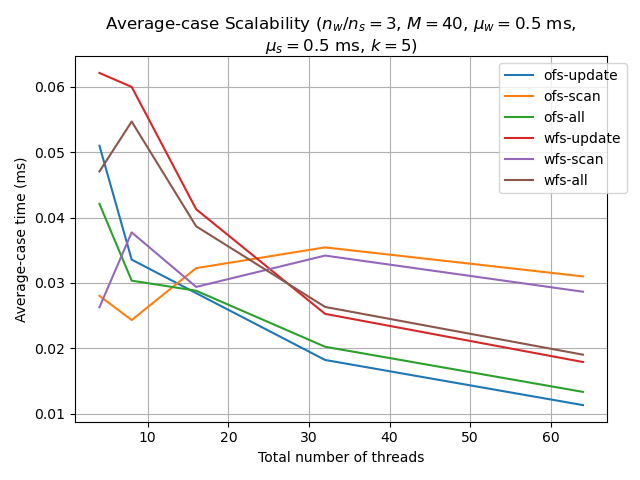
\includegraphics[width=\columnwidth]{images/exp1.png} 
    \caption{Average case scalability with varying number of threads.}
    \label{fig:exp1}
\end{figure}

\begin{figure}[!ht]
    \centering
    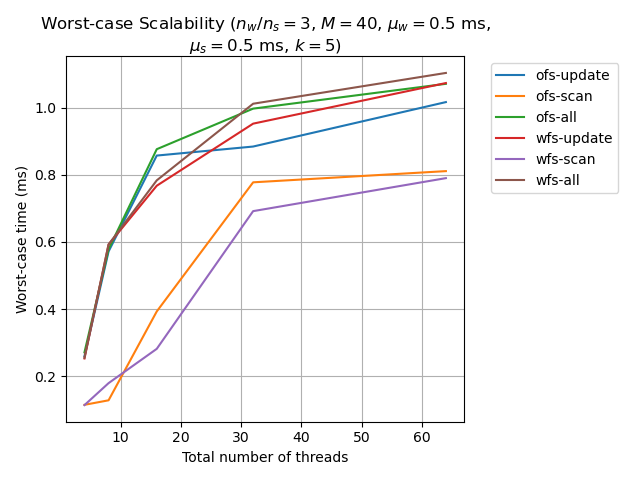
\includegraphics[width=\columnwidth]{images/exp2.png}
    \caption{Worst case scalability with varying number of threads.}
    \label{fig:exp2}
\end{figure}

We observe the following.
\begin{enumerate}
    \item In the average and worst case, the obstruction-free snapshot is
    approximately 4-5 times faster and more scalable than the wait-free
    snapshot.
    \item In the average and worst case, the update operation of the
    obstruction-free snapshot takes constant time while the update operation for
    the wait-free snapshot increases linearly with the number of threads. For
    both algorithms, the snapshot operation increases linearly with time.
    \item The gap between the times taken for the update and snapshot operation
    is huge for the obstruction-free snapshot and small for the wait-free
    snapshot. In fact, the update operation takes longer for the wait-free
    snapshot for a larger number of threads.
    \item The reason for poor performance and scalability of the wait-free
    snapshot is because of the fact that update threads have to perform a
    snapshot as well to ensure wait-free guarantees, which is not the case in
    the obstruction-free snapshot.
\end{enumerate}

\subsection{Impact of Update on Scan}
\label{susbec:impact-update-scan}

As the number of update threads per scan thread increases, there are more
threads that can obstruct the snapshot operation, thus we should expect the
snapshot operation to take longer for a larger \(\frac{n_w}{n_s}\), the number
of update to scan threads. The average and worst case analysis are shown in
\autoref{fig:exp3} and \autoref{fig:exp4}.

\begin{figure}[!ht]
    \centering
    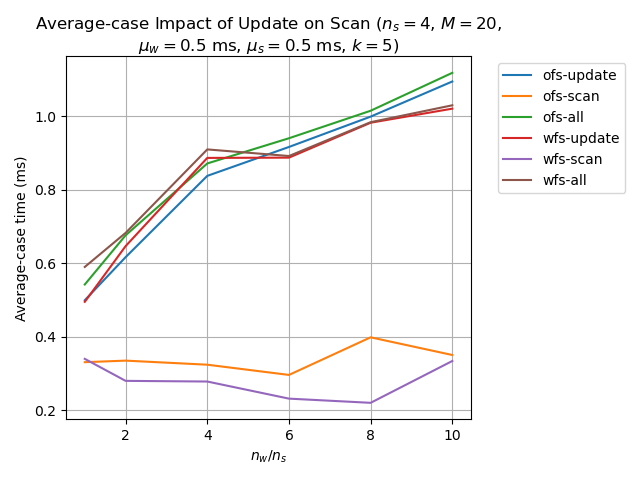
\includegraphics[width=\columnwidth]{images/exp3.png} 
    \caption{Average case impact of update on snapshot with varying \(\frac{n_w}{n_s}\).}
    \label{fig:exp3}
\end{figure}

\begin{figure}[!ht]
    \centering
    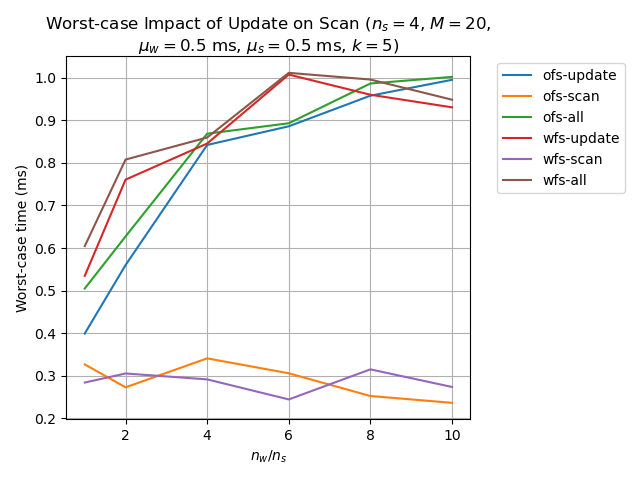
\includegraphics[width=\columnwidth]{images/exp4.png} 
    \caption{Worst case impact of update on snapshot with varying \(\frac{n_w}{n_s}\).}
    \label{fig:exp4}
\end{figure}

We observe the following.
\begin{enumerate}
    \item For the wait-free implementation, the average and worst case runtimes
    for each operation increases with the ratio \(\frac{n_w}{n_s}\). The runtime
    remains constant for the obstruction-free snapshot.
    \item For the obstruction-free snapshot, snapshot operation is a bottleneck,
    but for the wait-free snapshot, update operation is a bottleneck (since a
    snapshot operation is also performed).
    \item Though there are no wait-free guarantees for the obstruction-free
    snapshot, it proves to be faster in practice due to the lightweight update
    operation. Another reason for no obstruction is probably due to the
    exponential sleep time.
\end{enumerate}

\section{Conclusion}
\label{sec:conclusion}

From the analysis, we conclude that even though there are no wait-free
guarantees, the obstruction-free snapshot algorithm performs much better than
the wait-free snapshot algorithm. This might be due to smaller size of the
shared array. An analysis with a larger shared array may be required to fully
assess the speed of the obstruction-free snapshot algorithm in practice.

\end{document}